\chapter{Extração de características e classificação}
\label{cp:6_extracao}
Para que o sistema biométrico possa realizar a identificação dos indivíduos é necessário que existam técnicas para extração das características e logo em seguida suas respectivas classificações. Deste modo neste capítulo são apresentadas as técnicas para extração e classificação das características utilizadas neste trabalho.

Como estratégia de extração de características foi utilizada a Transformada Wavelet (TW), já na tarefa de classificação aplicou-se os classificadores K-vizinhos mais próximos (do inglês: \textit{K Nearest Neighbors} - KNN), Máquina de Aprendizado Extremo (do inglês: \textit{Extreme Learning Machine} - ELM) e Máquinas de Vetores de Suporte (do inglês: \textit{Support Vector Machine} - SVM). Os quais estão descritos com mais detalhes nas seções abaixo. 

\section{Transformada Wavelet}
\label{sec:Transformada Wavelet}
Para extração das características, foi aplicada a TW \cite{mallat1989theory} que é considerada uma técnica de processamento de sinal que atua tanto no domínio da frequência como no domínio do tempo diferentemente da Transformada de Fourier que atua apenas no domínio do tempo. É uma técnica muito utilizada para extração de características seja de um sinal por meio de decomposições 1D ou de uma imagem por meio de decomposições 2D. Aplicando as decomposições seja em um sinal ou uma imagem são gerados alguns elementos chamados coeficientes que podem ser de baixa e alta frequência e que representam, respectivamente, detalhes e aproximações dos dados originais. 

Essa abordagem utiliza um conjunto de filtros de suavização de imagem, sendo um filtro passa-baixa \textit{g}, que representa uma aproximação do sinal original e um filtro passa-alta \textit{h}, representando os detalhes. Como as imagens são dados bidimensionais,
após a decomposição Wavelet 2D são geradas quatro subimagens, cada  uma delas de dimensão  $(\frac{n}{2} \times$  $\frac{n}{2})$. Alguns autores chamam de \textit{down-sampling} o processo de diminuição das dimensões da imagem, esse processo sendo representado pelas setas para baixo conforme a figura \ref{fig:wavelet}. Seguindo esse contexto, supondo que a imagem a ser extraída a característica possui dimensão (256 $\times$ 256) pixels, ao final as subimagens geradas possuem dimensão (128 $\times$ 128) pixels, sendo originadas por meio da aplicação dos filtros passa-baixa e passa-alta nas linhas e colunas da imagem.


 Na figura \ref{fig:wavelet} é apresentada uma rápida ilustração dos passos de decomposição da Wavelet 2D com as quatro subimagens sendo elas: (\textit{i}) LL (aproximação); (\textit{ii}) HL (detalhes horizontais); (\textit{iii}) LH (detalhes verticais); e (\textit{iv})HH (detalhes diagonais). De tal modo que a imagem LL representa apenas uma aproximação da imagem original. 









\begin{figure}[H]
\centering
\caption{Estrutura de uma Transformada Wavelet}
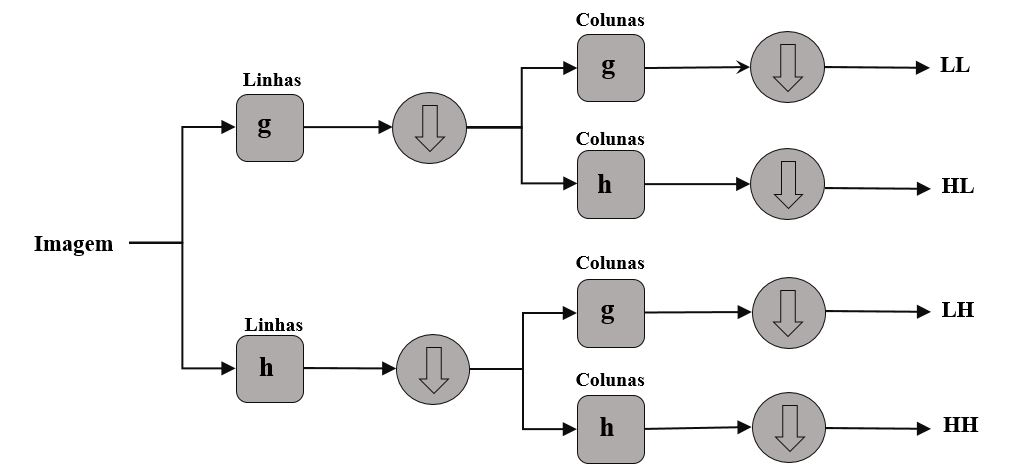
\includegraphics[scale =0.62]{imgs/decomposicao2d.png}
\source{Jonas Mendonça Targino, 2018}
\label{fig:wavelet}
\end{figure}

Na figura \ref{fig:imgsWavelet} é apresentada um exemplo de subimagens geradas por meio da Transformada Wavelet 2D (LL, HL, LH e HH), ao final esse conjunto de coeficientes pode ser utilizado para representar a imagem original.  Costuma-se utilizar os componentes da imagem LL do nível 3, que representa uma aproximação da imagem original e apresenta menor dimensão e boa representatividade, como relatado no trabalho de  \citeonline{costa2011ensemble}.

\begin{figure}[H]
\centering
\caption{Imagens obtidas após a decomposição Wavelet 2D }
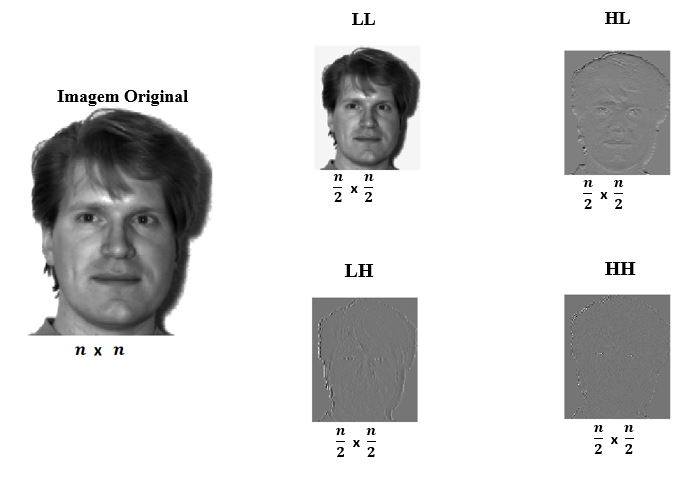
\includegraphics[scale =0.75]{imgs/tw.png}
\source{Jonas Mendonça Targino, 2018. Imagem de face obtida da base Yale \cite{georghiades1997yale}}
\label{fig:imgsWavelet}
\end{figure}



\section{K-Vizinhos mais próximos}


O KNN é um algoritmo proposto a mais de seis décadas, sendo bastante utilizado e estudado para a tarefa de reconhecimento de padrões. De maneira que seu núcleo de funcionamento está em descobrir o vizinho mais próximo de um determinado ponto. Podendo encontrar os $K$ vizinhos mais próximos de um ponto de consulta, em vez de utilizar apenas o primeiro vizinho mais próximo.

A ideia geral do KNN é classificar um dado elemento a partir da análise das respectivas classes dos \textit{K} vizinhos mais próximos pertencentes ao conjunto de treinamento. Essa técnica calcula a distância do ponto de consulta para  cada elemento do conjunto de treinamento. Após esse cálculo, todas as distâncias são ordenadas em ordem crescente do elemento mais próximo ao mais distante.

Após os elementos ordenados, são selecionados os $K$ primeiros, os quais são utilizados para a tarefa de classificação. Exemplo: 1-NN utiliza-se o $K$ = 1, ou seja, utilizamos o primeiro elemento do conjunto de treinamento, aquele que apresenta menor distância. Já o 6-NN vai utilizar os seis vizinhos mais próximos, e com  base nos votos majoritários do seis vizinhos mais próximos infere-se a classe do elemento de consulta. É possível visualizar na figura \ref{fig:knn} um exemplo de classificação com K-NN, de modo que $K$ = 6.

\begin{figure}[ht]
\centering
\caption{Exemplo de classificação do K-NN com duas classes e K = 6}
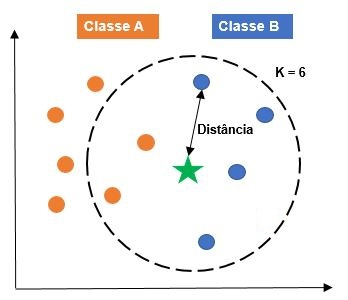
\includegraphics[scale=0.9]{imgs2/knn.png}
\source{Jonas Mendonça Targino, 2018}

\label{fig:knn}
\end{figure}


A literatura apresenta muitas aplicações usando KNN, como o diagnóstico de câncer de mama \cite{Sarkar_2000}, a classificação de texto \cite{Yu_2007} e \cite{Han_2001}, reconhecimento de emoção \cite{Cheng_2008}, identificação de falante \cite{Kacur_2011} , entre muitos outros. 

Uma das principais fraquezas do classificador KNN é que todas as amostras de treinamento devem ser armazenadas na memória e, para realizar a classificação, é necessário o cálculo da distância da amostra de teste para todas as amostras de treino.  À medida que o número de amostras no conjunto de treinamento aumenta, armazenar todos os seus valores na memória do computador pode não ser viável e também o procedimento de classificação pode levar muito tempo devido o cálculo das distâncias.


%\section{Rede Neural MLP}
%Uma rede neural é uma estrutura computacional inspirada no estudo do processamento neural biológico. Existem muitos tipos diferentes de redes neurais, de relativamente simples a muito complexas, assim como existem muitas teorias sobre o funcionamento do processamento neural biológico. Uma rede neural de alimentação avançada em camadas tem camadas ou subgrupos de elementos de processamento. Uma camada de elementos de processamento faz cálculos independentes em dados que recebe e passa os resultados para outra camada. A próxima camada pode, por sua vez, fazer seus cálculos independentes e transmitir os resultados para outra camada. Finalmente, um subgrupo de um ou mais elementos de processamento determina a saída da rede. Cada elemento de processamento faz seu cálculo com base em uma soma ponderada de suas entradas. A primeira camada é a camada de entrada e a última camada de saída. As camadas que são colocadas entre as primeiras e as últimas camadas são as camadas ocultas. Os elementos de processamento são vistos como unidades que são semelhantes aos neurônios em um cérebro humano e, portanto, são referidas como células ou neurônios artificiais. Uma função de limite é às vezes usada para qualificar a saída de um neurônio na camada de saída. As sinapses entre neurônios são referidas como conexões, que são representadas por bordas de um gráfico direcionado em que os nós são os neurônios artificiais. As redes neurais consistem em pequenas unidades chamadas neurônios, e estas estão conectadas entre si de tal maneira que podem passar sinais uns dos outros \cite{Askarunisa_2009}.
%
%Um percorridor de camada única avançado treinado com Back-propagation e Levenberg-Marquardt algoritmo \cite{haykin_2009}, foi usado neste trabalho. O algoritmo Back-propagation usado no treinamento de perceptron multicamada, é formulado como um problema não linear de mínimos quadrados. Essencialmente, o algoritmo de Levenberg-Marquardt é um método de estimativa de mínimos quadrados baseado na ideia máxima de vizinhança. Deixe $ E (w) $ ser uma função de erro objetivo composta de $ m $ termos de erro individual $ e_i ^ 2 (w) $ como segue:
%\[E (w) = \ sum_ {i = 1} ^ m e_i ^ 2 (w) = || f (w) || ^ 2 \]
%Em que
%\[e_i ^ 2 (w) = (y_ {i} -y_ {ri}) ^ 2 \]
%$ y_ {i} $ é o valor desejado do neurônio de saída $ i $ e $ y_ {ri} $ é a saída real desse neurônio. Supõe-se que a função $ f (.) $ E o Jacobiano $J$ são conhecidos no ponto $ w $. O objetivo do algoritmo Levenberg-Marquardt é calcular o vetor de peso $ w $, de modo que $ E (w) $ seja mínimo. Em cada iteração, o vetor de peso é atualizado de acordo com (\ ref {eq: atualizaw}).
%
%\begin{equation}
%\label{eq:atualizaw}
%w_{k+1}=w_k + \delta w_k
%\end{equation}
%em que
%\begin{equation}
%\label{eq:gradiente}
%\delta w_k = - (J_k^Tf(w_k))(J_k^TJ_k+ \lambda I)^{-1}
%\end{equation}
%$ J_k $ é a jacobiana de $ f (.) $ Avaliado em $ w_k $, $ \lambda $ é o parâmetro Marquardt e $ I $ é a matriz de identidade.
%
%
%
%
%\section{Floresta de caminhos ótimos}
%Ao contrário do k-NN, o OPF é um classificador muito recente proposto nos anos 2000 por \cite{Papa_2009a}. Não é paramétrico, rápido, simples, multi-classe, não faz qualquer suposição sobre as formas das classes e pode lidar com qualquer grau de sobreposição entre classes \cite{Papa_2009a}. O OPF foi usado com sucesso em muitas aplicações, como a detecção de patologia laríngea \cite{Papa_2008}, reconhecimento de face \cite{Papa_2009b}, estimativa de chuva \cite{Freitas_2009}, categorização de imagem \cite{Papa_2011}, entre muitos outros.
%
%
%O OPF é uma técnica de classificação baseada em gráficos, sendo responsável pela redução, para classificar cada classe, ou seja, o protótipo de acordo com uma ou mais árvores. Portanto, cada nó do gráfico representa uma amostra do conjunto de treinamento atuando mais especificamente como o descritor, pertencente à árvore do protótipo, na medida em que é maior grau de conexão de acordo com as bordas que são as distâncias entre os descritores.




\section{Máquina de aprendizado extremo}
\label{sec:ELM}

Máquina de Aprendizado Extremo é um algoritmo de classificação proposto por  \cite{Huang_2006} e \cite{Huang_2009}. A ELM é uma rede neural artificial (RNA) com uma única camada oculta, essa estratégia vem alcançando sucesso no contexto de classificação e regressão. 

A ELM possui o mesmo princípio de funcionamento de uma RNA,   diferenciando-se da MLP e RBF por sua metodologia de treinamento que não é baseada em gradientes. Isso deve-se ao fato que a ELM atualiza apenas os pesos da camada escondida. Já os pesos da camada de entrada são escolhidos aleatoriamente e fixados, isso permite a essa estratégia escapar das principais deficiências do algoritmo de treinamento \textit{backpropagation}. Possibilitando velocidade de aprendizado significativamente rápida, quando comparada a redes neurais MLP e RBF, assim como também proporciona menor intervenção humana do que outros algoritmos. Outro ponto é a facilidade e rapidez na implementação quando comparada a implementação de outros classificadores tradicionais.

A ELM pode determinar analiticamente todos os parâmetros de uma rede neural MLP em vez de ajustar parâmetros iterativamente. Assim, podendo superar algumas das dificuldades do método baseado em gradientes e da maioria dos outros métodos de aprendizagem. O trabalho de \cite{Huang_2006} também mostra que a ELM tende alcançar melhores resultados de generalização do que técnicas de classificação como SVM. Outro fator importante da ELM é sua baixa sensibilidade aos parâmetros especificados pelo usuário. Na figura \ref{fig:ELM} é possível visualizar a estrutura de uma ELM.

\begin{figure}[H]
\centering
\caption{Estrutura de uma Rede Neural ELM}
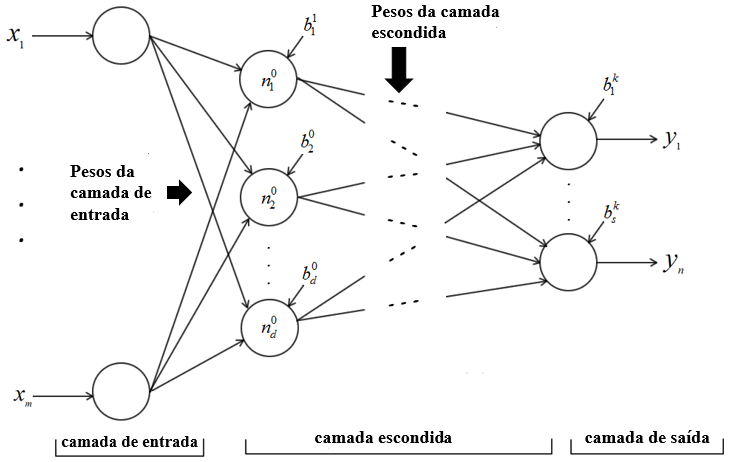
\includegraphics[scale=0.60]{imgs/ELM.png}
\source{Jonas Mendonça Targino, 2018}
\label{fig:ELM}
\end{figure}



No treinamento da ELM a matriz \textbf{W} (pesos da camada de entrada) é gerada de maneira aleatória e é inalterada. Portanto, o objetivo do treinamento da ELM é encontrar a matriz de pesos $\beta$, que são os pesos da camada oculta, baseado na matriz de saída \textbf{Y} e na matriz de pesos aleatórios \textbf{W}, por meio da resolução de um sistema linear. 

Com essa finalidade, a primeira ação é determinar \textbf{H}, que é a matriz que contem a função de ativação (podendo ser sigmóide, tangente hiperbólica, e etc.) dos neurônios da camada oculta.  Portanto, a matriz \textbf{H} armazena o resultado de todos os neurônios da camada oculta obtidos a partir da multiplicação entre \textbf{X} e \textbf{W}. Após determinada a matriz \textbf{H}, para se obter os pesos da matriz $\beta$ deve ser solucionado o sistema linear presente na equação \ref{eq:pinv}.


\begin{equation}
H = f_{ativ}(X\cdot W) \Rightarrow H\boldsymbol{\mathbf{\beta}} = Y \Rightarrow \mathbf{\mathbf{B}} = pinv(H)\cdot Y
\label{eq:pinv}
\end{equation}

Em que $f_{ativ}$ é a função de ativação e \textit{pinv} é pseudo inversa da matriz H. 



\section{Máquina de vetores suporte}
\nomenclature{SVM}{Support Vector Machines}
A Máquina de Vetores Suporte \cite{cortes1995support}  funciona da seguinte forma: dado um conjunto de dados de treinamento composto de \textit{N} amostras $\{x_i, y_i \}_{i = 1} ^ N $ com entrada $ x_i \in \mathcal{R}^n$ e saída $y_i \in \pm 1 $, o classificador SVM visa construir uma superfície de decisão da forma $ sign [f (x; w)] $, em que 
$ f (x; w) = w ^ T \phi (x) + b $
é uma aproximação da função de mapeamento $ y $, $ w \in \mathcal {R} ^ m $ e $ \ phi (.): \mathcal {R}^n \rightarrow \mathcal {R}^m $ is uma função que mapeia a entrada para um espaço de recurso de dimensão superior chamado. O parâmetro $ w $ e $ b $ podem ser obtidos por meio do seguinte problema de otimização \cite{Vapnik}:

\begin{equation}
\label {eq: rule1}
\min_ {w, b, \xi} \Phi (w, b, \xi) = \frac{1}{2} (w^Tw) + C \sum_ {i = 1} ^ N \xi_i,
\end{equation}

\noindent sujeito a $ y_i [w ^ T \phi (x_i) + b]\ geq 1 - \xi_i, \xi_i \geq 0, i = 1, \cdots, N $, em que $ C $ é um \textit{trade-off} parâmetro que indica a importância relativa da complexidade do modelo quando comparado ao erro de treinamento e $ \xi_i $ é o erro de treinamento para a amostra $ i $ -th.
Por simplicidade, o problema (\ref{eq: rule1}) geralmente é convertido em um problema equivalente definido em um espaço duplo, construindo o seguinte Lagrangiano \cite{Vapnik}: $ L (w, b, \xi, \beta, \gamma) $.

\begin{equation}
\frac {1} {2} w ^ Tw + C \sum_ {i = 1} ^ N \xi_i- \sum_ {i = 1} ^ N \beta_i \{[w ^T \phi (x_i) + b] y_i-1 + \ xi_i \} - \sum_{i = 1} ^ N \gamma_i \ xi_i
\end{equation}

\noindent em que $ \beta_i \geq 0 $, $ \gamma_i \geq 0 $, $ (i = 1, \cdots, N) $ são multiplicadores Lagrange. Em tal informação, um determinado tipo de função, conhecido como kernel, é empregado \cite{Scholkopf}. Deve seguir a restrição imposta pelo Teorema de Mercer e fornece um cálculo implícito de um passo do produto entre $ \phi (x_i) $ e $ \ phi (x_j) $: $ K (x_i, x_j) = <\phi (x_i), \phi (x_j)> $. Os resultados discutidos na Seção \ ref {seg: resultados} foram obtidos com o Kernel RBF: $ K (x_i, x_j) = exp \left (- \frac {(x_i-x_j) ^ T (x_i-x_j)} {2 \sigma ^ 2} \right) $, em que $ \sigma ^ 2 $ indica a variância a ser definida pelo usuário. Usando o Kernel, $f(x; w) $ podem ser reescritos como
$ f (x; w) = \sum_{i = 1} ^ N \beta_iy_iK(x, x_i) + b $.

Para as amostras de treino ao longo do limite de decisão, os correspondentes $ \alpha_i $ são maiores do que zero, conforme estabelecido pelo teorema de Karesh-Kuhn-Tucker. Essas amostras são conhecidas como vetores de suporte. O número de vetores de suporte geralmente é muito menor que $ N $, sendo proporcional ao erro de generalização do classificador. O vetor de teste $ {x}$ em $ {R} ^ m $ é atribuído a uma determinada classe de acordo com $ f(n) = sign [\mathbf {w} ^ T \phi (\mathbf {x}) + b] = sign(\sum_ {i = 1} ^ {N} \alpha_iy_iK (\mathbf {x}, \mathbf {x_i}) + b) $.  Podemos visualizar o problema de classificação binário por meio da figura \ref{fig:svm}.

\begin{figure}[H]
\centering
\caption{Problema de classificação binário com SVM}
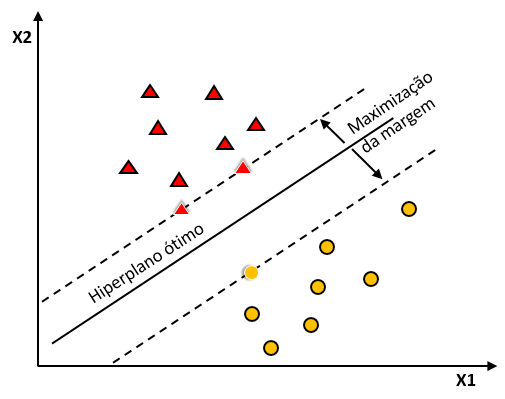
\includegraphics[scale=0.60]{imgs/svm}
\source{Jonas Mendonça Targino, 2018}
\label{fig:svm}
\end{figure}


\section{Considerações finais do capítulo}

Existe uma quantidade considerável de classificadores e extratores presentes na literatura, entretanto neste trabalho foi utilizada a Transformada Wavelet como extrator de características, enquanto como classificadores utilizou-se K-vizinhos mais próximos, Máquina de Aprendizado Extremo e Máquinas de Vetores de Suporte. 
